\documentclass[../DoAn.tex]{subfiles}
\begin{document}

\section{Thiết kế kiến trúc}
\subsection{Lựa chọn kiến trúc phần mềm}
Mục này có độ dài từ một đến ba trang. Sinh viên cần lựa chọn kiến trúc phần mềm cho ứng dụng của mình như: kiến trúc ba lớp MVC, MVP, SOA, Microservice, v.v. rồi giải thích sơ bộ về kiến trúc đó (không giải thích chi tiết/dài dòng).
Sử dụng kiến trúc phần mềm đã chọn ở trên, sinh viên mô tả kiến trúc cụ thể cho ứng dụng của mình. Gợi ý: sinh viên áp dụng lý thuyết chung vào hệ thống/sản phẩm của mình như thế nào, có thay đổi, bổ sung hoặc cải tiến gì không. Ví dụ, thành phần M trong kiến trúc lý thuyết MVC sẽ là những thành phần cụ thể nào (ví dụ: là interface I + class C1 + class C2, v.v.) trong kiến trúc phần mềm của sinh viên.

\subsection{Thiết kế tổng quan}
Sinh viên vẽ biểu đồ gói UML (UML package diagram), nêu rõ sự phụ thuộc giữa các gói (package). SV cần vẽ các gói sao cho chúng được phân theo các tầng rõ ràng, không được sắp đặt package lộn xộn trong hình vẽ. Sinh viên chú ý các quy tắc thiết kế (Các gói không phụ thuộc lẫn nhau, gói tầng dưới không phụ thuộc gói tầng trên, không phụ thuộc bỏ qua tầng, v.v.) và cần giải thích sơ lược về mục đích/nhiệm vụ của từng package. SV tham khảo ví dụ minh họa trong Hình \ref{fig:Fig1}
\begin{figure}[H]
    \centering
    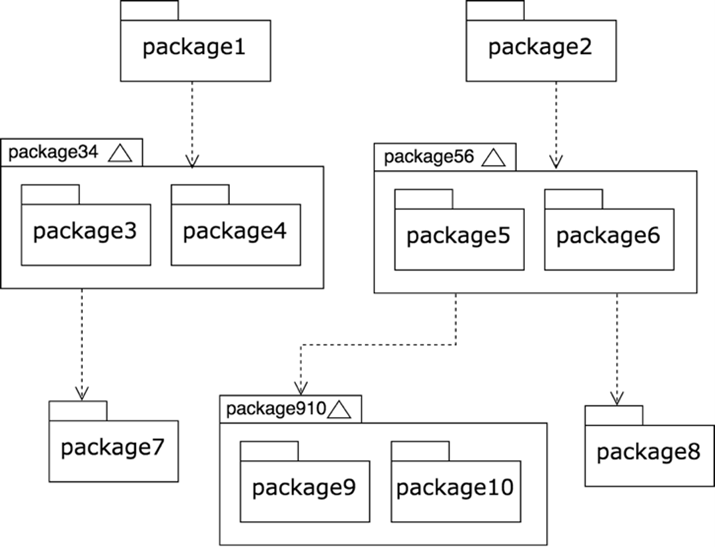
\includegraphics{Hinhve/Picture1.png}
    \caption{Ví dụ biểu đồ phụ thuộc gói}
    \label{fig:Fig1}
\end{figure}
\subsection{Thiết kế chi tiết gói}
Sinh viên thiết kế và lần lượt vẽ biểu đồ thiết kế cho từng package, hoặc một nhóm các package liên quan để giải quyết một vấn đề gì đó. Khi vẽ thiết kế gói, sinh viên chỉ cần đưa tên lớp, không cần chỉ ra các thành viên phương thức và thuộc tính. SV tham khảo ví dụ minh họa trong Hình \ref{fig:Fig2}.

Sinh viên cần vẽ rõ ràng quan hệ giữa các lớp trong biểu đồ. Các quan hệ bao gồm: phụ thuộc (dependency), kết hợp (association), kết tập (aggregation), hợp thành (composition), kế thừa (inheritance), và thực thi (implementation). Các quan hệ này đều đã được minh họa trong \ref{fig:Fig2}.

Sau khi vẽ hình minh họa, sinh viên cần giải thích ngắn gọn về thiết kế của mình. 

\begin{figure}[H]
    \centering
    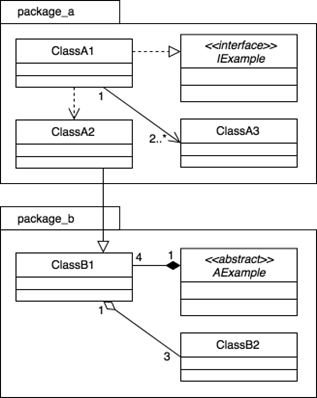
\includegraphics{Hinhve/Picture2.png}
    \caption{Ví dụ thiết kế gói}
    \label{fig:Fig2}
\end{figure}

\section{Thiết kế chi tiết}
\subsection{Thiết kế giao diện}
Phần này có độ dài từ hai đến ba trang. Sinh viên đặc tả thông tin về màn hình mà ứng dụng của mình hướng tới, bao gồm độ phân giải màn hình, kích thước màn hình, số lượng màu sắc hỗ trợ, v.v. Tiếp đến, sinh viên đưa ra các thống nhất/chuẩn hóa của mình khi thiết kế giao diện như thiết kế nút, điều khiển, vị trí hiển thị thông điệp phản hồi, phối màu, v.v. Sau cùng sinh viên đưa ra một số hình ảnh minh họa thiết kế giao diện cho các chức năng quan trọng nhất. Lưu ý, sinh viên không nhầm lẫn giao diện thiết kế với giao diện của sản phẩm sau cùng.
\subsection{Thiết kế lớp}
Phần này có độ dài từ ba đến bốn trang. Sinh viên trình bày thiết kế chi tiết các thuộc tính và phương thức cho một số lớp chủ đạo/quan trọng nhất của ứng dụng (từ 2-4 lớp). Thiết kế chi tiết cho các lớp khác, nếu muốn trình bày, sinh viên đưa vào phần phụ lục.

Để minh họa thiết kế lớp, sinh viên thiết kế luồng truyền thông điệp giữa các đối tượng tham gia cho 2 đến 3 use case quan trọng nào đó bằng biểu đồ trình tự (hoặc biểu đồ giao tiếp).
\subsection{Thiết kế cơ sở dữ liệu}
Phần này có độ dài từ hai đến bốn trang. Sinh viên thiết kế, vẽ và giải thích biểu đồ thực thể liên kết (E-R diagram). Từ đó, sinh viên thiết kế cơ sở dữ liệu tùy theo hệ quản trị cơ sở dữ liệu mà mình sử dụng (SQL, NoSQL, Firebase, v.v.)

\section{Xây dựng ứng dụng}
\subsection{Thư viện và công cụ sử dụng}
Sinh viên liệt kê các công cụ, ngôn ngữ lập trình, API, thư viện, IDE, công cụ kiểm thử, v.v. mà mình sử dụng để phát triển ứng dụng. Mỗi công cụ phải được chỉ rõ phiên bản sử dụng. SV nên kẻ bảng mô tả tương tự như Bảng \ref{table:my_label}. Nếu có nhiều nội dung trình bày, sinh viên cần xoay ngang bảng.

\begin{table}[H]
\centering{}
    \begin{tabular}{lll}
        \hline
        \textbf{Mục đích} & \textbf{Công cụ}       & \textbf{Địa chỉ URL}    \\ \hline
        IDE lập trình     & Eclipse Oxygen a64 bit & http://www.eclipse.org/ \\ \hline
        v.v.              & v.v.                   & v.v.                    \\ \hline
        \end{tabular}
    \caption{Danh sách thư viện và công cụ sử dụng}
    \label{fig:my_label}
\end{table}

\subsection{Kết quả đạt được}
Sinh viên trước tiên mô tả kết quả đạt được của mình là gì, ví dụ như các sản phẩm được đóng gói là gì, bao gồm những thành phần nào, ý nghĩa, vai trò?

Sinh viên cần thống kê các thông tin về ứng dụng của mình như: số dòng code, số lớp, số gói, dung lượng toàn bộ mã nguồn, dung lượng của từng sản phẩm đóng gói, v.v. Tương tự như phần liệt kê về công cụ sử dụng, sinh viên cũng nên dùng bảng để mô tả phần thông tin thống kê này.

\subsection{Minh họa các chức năng chính}
Sinh viên lựa chọn và đưa ra màn hình cho các chức năng chính, quan trọng, và thú vị nhất. Mỗi giao diện cần phải có lời giải thích ngắn gọn. Khi giải thích, sinh viên có thể kết hợp với các chú thích ở trong hình ảnh giao diện.

\section{Kiểm thử}
Phần này có độ dài từ hai đến ba trang. Sinh viên thiết kế các trường hợp kiểm thử cho hai đến ba chức năng quan trọng nhất. Sinh viên cần chỉ rõ các kỹ thuật kiểm thử đã sử dụng. Chi tiết các trường hợp kiểm thử khác, nếu muốn trình bày, sinh viên đưa vào phần phụ lục.
Sinh viên sau cùng tổng kết về số lượng các trường hợp kiểm thử và kết quả kiểm thử. Sinh viên cần phân tích lý do nếu kết quả kiểm thử không đạt.
\section{Triển khai}
Sinh viên trình bày mô hình và/hoặc cách thức triển khai thử nghiệm/thực tế. Ứng dụng của sinh viên được triển khai trên server/thiết bị gì, cấu hình như thế nào. Kết quả triển khai thử nghiệm nếu có (số lượng người dùng, số lượng truy cập, thời gian phản hồi, phản hồi người dùng, khả năng chịu tải, các thống kê, v.v.)

\end{document}
